\documentclass[a4paper]{article}
\usepackage[UTF8]{ctex}
\usepackage[a4paper,margin=1in]{geometry}
\usepackage{graphicx}
\usepackage{float}
\usepackage{listings}
\usepackage{booktabs}
\usepackage{hyperref}
\usepackage{fancyhdr}
\usepackage{lastpage}
\usepackage{color}
\usepackage{xcolor}
\usepackage{indentfirst}
\setlength{\parindent}{2em}
\usepackage{zhnumber}
\usepackage[dvipsnames]{xcolor}
\usepackage{amsmath}
\usepackage{tikz}
\usetikzlibrary{shapes,arrows,positioning}

% ===== 个人信息与实验信息配置 =====
\newcommand{\projname}{基于表达式的计算器 ExprEval}
\newcommand{\reporttitle}{实验4-设计文档}
\newcommand{\stuno}{23336179}
\newcommand{\authorname}{马福泉}
\newcommand{\major}{计算机科学与技术}
\newcommand{\adviser}{李文军}
\newcommand{\startdate}{2026年4月}
\newcommand{\labenddate}{2026年5月}
\newcommand{\labroom}{B203}

% ===== 页眉页脚设置 =====
\pagestyle{fancy}
\fancyhf{}
\fancyhead[L]{\kaishu \projname}
\fancyhead[C]{\kaishu \reporttitle}
\fancyhead[R]{\kaishu \authorname}
\fancyfoot[C]{第 \thepage 页，共 \pageref{LastPage} 页}
\renewcommand{\headrulewidth}{0.4pt}
\renewcommand{\footrulewidth}{0pt}

% ===== 代码高亮配置 (适应 Java) =====
\definecolor{NavyBlue}{RGB}{0,0,128}
\definecolor{codegreen}{RGB}{0,128,0}
\definecolor{codegray}{RGB}{128,128,128}
\definecolor{codepurple}{RGB}{128,0,128}
\definecolor{backcolour}{RGB}{245,245,245}

\lstset{
    language=Java,
    basicstyle=\ttfamily\small,
    commentstyle=\color{codegreen}\itshape,
    keywordstyle=\color{NavyBlue}\bfseries,
    stringstyle=\color{codepurple},
    numberstyle=\tiny\color{codegray},
    backgroundcolor=\color{backcolour},
    breaklines=true,
    frame=single,
    numbers=left,
    tabsize=4,
    showstringspaces=false,
    captionpos=b,
    escapeinside={\%}{\%},
    morekeywords={enum,record}
}

\begin{document}

% ==================== 封面 ====================
\begin{titlepage}
    \centering
    
    
\includegraphics[width=10cm]{img/SYSULogo.png}

    \vspace{1em}
    {\Large \kaishu \projname \par}
    \vspace{3em}

    {\fontsize{36pt}{40pt}\kaishu \selectfont \boldmath \reporttitle\par}
    \vspace{2em}
    \vspace*{\fill}

    \begin{center}
    {\Large
    \makebox[5em][s]{学号}:\underline{\makebox[15em][c]{\kaishu \stuno}}\\[1em]
    \makebox[5em][s]{姓名}:\underline{\makebox[15em][c]{\kaishu \authorname}}\\[1em]
    \makebox[5em][s]{专业}:\underline{\makebox[15em][c]{\kaishu \major}}\\[1em]
    \makebox[5em][s]{指导教师}:\underline{\makebox[15em][c]{\kaishu \adviser}}\\[1em]
    \makebox[5em][s]{起始日期}:\underline{\makebox[15em][c]{\kaishu \startdate}}\\[1em]
    \makebox[5em][s]{结束日期}:\underline{\makebox[15em][c]{\kaishu \labenddate}}\\[1em]
    \makebox[5em][s]{实验地点}:\underline{\makebox[15em][c]{\kaishu \labroom}}
    }
    \end{center}

    \vspace*{\fill}
\end{titlepage}

% ==================== 目录 ====================
\tableofcontents
\newpage

% ==================== 正文 ====================

% ========== 第1章 实验简述 ==========
\section{实验简述}

\subsection{实验目的}

本实验旨在实现一个基于表达式的科学计算器 \textbf{ExprEval}。与实验三的后缀表达式转换器相比，ExprEval 不仅需要将中缀表达式转换为后缀形式，还要求对表达式进行完整的词法分析、语法分析以及语义求值，最终返回计算结果。

通过本实验，能够深入理解编译原理中以下核心概念：
\begin{enumerate}
    \item \textbf{词法分析（Lexical Analysis）}：使用确定性有限状态自动机（DFA）将字符流转换为 Token 流；
    \item \textbf{语法分析（Syntax Analysis）}：使用算符优先分析（Operator Precedence Parsing, OPP）将 Token 流构建为语法树并同步求值；
    \item \textbf{语义分析（Semantic Analysis）}：在归约过程中进行类型检查和错误检测；
    \item \textbf{异常处理}：设计完整的三层异常体系，精确报告各种词法、语法和语义错误。
\end{enumerate}

\subsection{实验内容}

实现一个完整的表达式计算器，支持以下特性：

\begin{itemize}
    \item \textbf{数值类型}：整数、小数、科学记数法（如 \texttt{1.2e-3}、\texttt{2.25E+2}）
    \item \textbf{布尔常量}：\texttt{true}、\texttt{false}
    \item \textbf{算术运算符}：\texttt{+}、\texttt{-}（含一元取负）、\texttt{*}、\texttt{/}、\texttt{\^}
    \item \textbf{关系运算符}：\texttt{<}、\texttt{>}、\texttt{<=}、\texttt{>=}、\texttt{==}、\texttt{!=}
    \item \textbf{逻辑/位运算符}：\texttt{\&}、\texttt{|}、\texttt{!}、\texttt{\textasciitilde}
    \item \textbf{三元条件运算符}：\texttt{?:}
    \item \textbf{预定义函数}：\texttt{sin}、\texttt{cos}、\texttt{tan}、\texttt{log}、\texttt{sqrt}、\texttt{abs}、\texttt{pow}、\texttt{max}、\texttt{min}（共9个）
    \item \textbf{括号嵌套}：支持任意深度的括号表达式
\end{itemize}

\subsection{开发环境}

\begin{itemize}
    \item 操作系统：Windows 11
    \item 语言与工具：Java（JDK 1.5+ 兼容） + VS Code
    \item 构建：批处理脚本 \texttt{build.bat}
    \item 测试框架：XML 驱动的自动化回归测试
    \item 文档：LaTeX + \texttt{design.tex}
\end{itemize}

% ========== 第2章 分析与设计 ==========
\section{分析与设计}

\subsection{BNF 语法的二义性分析}

实验手册第 2.3.1 小节以标准 BNF 定义了输入表达式的形式化语法。经分析，该语法定义\textbf{存在二义性}，主要体现在以下三个方面。

\subsubsection{运算符优先级的二义性}

BNF 产生式是纯语法的，并未编码运算符优先级信息。例如产生式：
\begin{center}
\texttt{ArithExpr → ArithExpr + ArithExpr | ArithExpr * ArithExpr}
\end{center}
对于输入 \texttt{1 + 2 * 3}，可以推导出两棵不同的语法树：
\begin{itemize}
    \item 先将 \texttt{1 + 2} 归约为 \texttt{ArithExpr}，再与 \texttt{* 3} 结合 → 结果为 9
    \item 先将 \texttt{2 * 3} 归约为 \texttt{ArithExpr}，再与 \texttt{1 +} 结合 → 结果为 7
\end{itemize}
这是典型的"运算符优先级歧义"——BNF 自身无法区分 \texttt{+} 与 \texttt{*} 的执行次序。

\subsubsection{一元取负与二元减法的重载二义性}

BNF 中同时存在两条以 \texttt{-} 为核心的产生式：
\begin{itemize}
    \item \texttt{ArithExpr → – ArithExpr}（一元取负，优先级 9）
    \item \texttt{ArithExpr → ArithExpr – ArithExpr}（二元减法，优先级 6）
\end{itemize}
对于输入 \texttt{2 - 3 * -4}，扫描到第二个 \texttt{-} 时，仅凭 BNF 无法判断应展开为一元取负还是二元减法。

\subsubsection{三元运算符的结构二义性}

类似经典的"悬空 else"问题，BNF 中的三元产生式：
\begin{center}
\texttt{ArithExpr → BoolExpr ? ArithExpr : ArithExpr}
\end{center}
对于嵌套输入如 \texttt{a ? b ? c : d : e}，存在两种解释：
\begin{itemize}
    \item \texttt{a ? (b ? c : d) : e}（右结合，与 C 语言一致）
    \item \texttt{(a ? b) : (c ? d : e)}（非标准结合）
\end{itemize}

\subsubsection{二义性的解析方案}

本实验采用\textbf{算符优先分析（OPP）}技术消解上述所有二义性：

\begin{enumerate}
    \item \textbf{优先级驱动}：通过 10 级优先关系表（参见表~\ref{tab:precedence}），\texttt{*} 优先级（7）高于 \texttt{+}（6），比较优先级时自动归约高优先级算符，从而保证 \texttt{1 + 2 * 3} 先算乘法。
    
    \item \textbf{上下文判别一元/二元减}：Scanner 阶段统一标记 \texttt{-} 为 \texttt{TokenType.SUB}。Parser 阶段通过布尔标志"前驱是操作数"判定：若前一 Token 为空/运算符/左括号，则识别为 \texttt{NEG}（一元取负）；否则为 \texttt{"-"}（二元减法）。
    
    \item \textbf{结合性规则}：优先关系表的结合性列明确标注右结合算符（如 \texttt{\^}、\texttt{?:}、\texttt{NEG}）。当栈顶与输入算符优先级相等时，右结合则移进，左结合则归约，从而将 \texttt{a ? b ? c : d : e} 解析为右结合形式。
\end{enumerate}

通过上述三种机制的组合，OPP 在不修改原始 BNF 的前提下高效消解了所有二义性，同时保证了分析器只需单遍扫描即可完成语法分析和语义求值。

\subsection{整体架构}

ExprEval 采用经典的"词法 → 语法 → 语义"三阶段流水线架构：

\begin{figure}[H]
\centering
\begin{tikzpicture}[node distance=1.5cm, auto,
    block/.style={rectangle, draw, text width=3cm, text centered, minimum height=1.2cm, fill=blue!10},
    arrow/.style={->, >=stealth, thick}]

    \node[block] (input) {输入表达式\\\texttt{String expression}};
    \node[block, right=of input] (scanner) {\texttt{Scanner}\\词法分析（DFA）};
    \node[block, right=of scanner] (parser) {\texttt{Parser}\\语法分析（OPP）};
    \node[block, right=of parser] (output) {计算结果\\\texttt{double}};
    \node[block, below=of scanner] (exceptions) {异常体系\\14 个异常类};

    \draw[arrow] (input) -- (scanner);
    \draw[arrow] (scanner) -- node[above] {Token流} (parser);
    \draw[arrow] (parser) -- (output);
    \draw[arrow, dashed] (scanner) -- (exceptions);
    \draw[arrow, dashed] (parser) -- (exceptions);

\end{tikzpicture}
\caption{ExprEval 系统架构}
\label{fig:architecture}
\end{figure}

调用入口 \texttt{Calculator.calculate(String)} 串联整个流程：
\begin{enumerate}
    \item 构造 \texttt{Scanner}，对输入字符串进行词法分析；
    \item 构造 \texttt{Parser}，使用 Scanner 提供的 Token 流进行算符优先分析；
    \item Parser 在归约过程中同步求值，返回最终结果（double）。
\end{enumerate}

\subsection{异常体系设计}

采用三层异常层次结构，自顶向下分别为通用的 \texttt{ExpressionException}、三大类别中间异常、以及具体异常子类：

\begin{figure}[H]
\centering
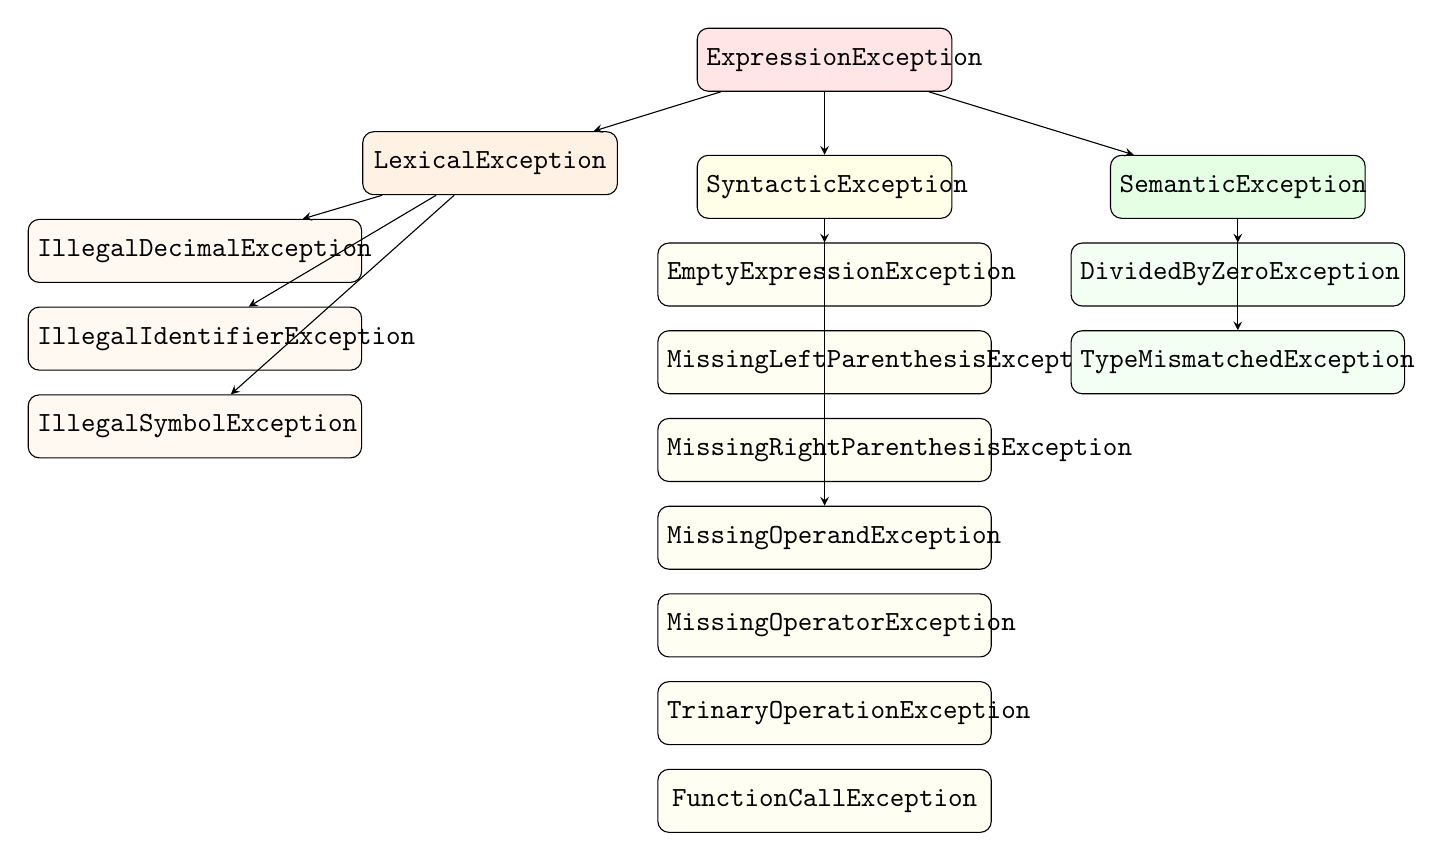
\begin{tikzpicture}[node distance=1.8cm, auto,
    block/.style={rectangle, draw, text width=3cm, text centered, minimum height=0.8cm, rounded corners}]

    \node[block, fill=red!10] (root) {\texttt{ExpressionException}};
    \node[block, fill=orange!10, below left=0.5cm and 1cm of root] (lex) {\texttt{LexicalException}};
    \node[block, fill=yellow!10, below=0.8cm of root] (syn) {\texttt{SyntacticException}};
    \node[block, fill=green!10, below right=0.8cm and 2cm of root] (sem) {\texttt{SemanticException}};

    \node[block, fill=orange!5, below left=0.3cm and 0cm of lex, text width=4cm] (lex1) {\texttt{IllegalDecimalException}};
    \node[block, fill=orange!5, below=0.3cm of lex1, text width=4cm] (lex2) {\texttt{IllegalIdentifierException}};
    \node[block, fill=orange!5, below=0.3cm of lex2, text width=4cm] (lex3) {\texttt{IllegalSymbolException}};

    \node[block, fill=yellow!5, below=0.3cm of syn, text width=4cm] (syn1) {\texttt{EmptyExpressionException}};
    \node[block, fill=yellow!5, below=0.3cm of syn1, text width=4cm] (syn2) {\texttt{MissingLeftParenthesisException}};
    \node[block, fill=yellow!5, below=0.3cm of syn2, text width=4cm] (syn3) {\texttt{MissingRightParenthesisException}};
    \node[block, fill=yellow!5, below=0.3cm of syn3, text width=4cm] (syn4) {\texttt{MissingOperandException}};
    \node[block, fill=yellow!5, below=0.3cm of syn4, text width=4cm] (syn5) {\texttt{MissingOperatorException}};
    \node[block, fill=yellow!5, below=0.3cm of syn5, text width=4cm] (syn6) {\texttt{TrinaryOperationException}};
    \node[block, fill=yellow!5, below=0.3cm of syn6, text width=4cm] (syn7) {\texttt{FunctionCallException}};

    \node[block, fill=green!5, below=0.3cm of sem, text width=4cm] (sem1) {\texttt{DividedByZeroException}};
    \node[block, fill=green!5, below=0.3cm of sem1, text width=4cm] (sem2) {\texttt{TypeMismatchedException}};

    \draw[->, >=stealth] (root) -- (lex);
    \draw[->, >=stealth] (root) -- (syn);
    \draw[->, >=stealth] (root) -- (sem);
    \draw[->, >=stealth] (lex) -- (lex1);
    \draw[->, >=stealth] (lex) -- (lex2);
    \draw[->, >=stealth] (lex) -- (lex3);
    \draw[->, >=stealth] (syn) -- (syn1);
    \draw[->, >=stealth] (syn) -- (syn4);
    \draw[->, >=stealth] (sem) -- (sem1);
    \draw[->, >=stealth] (sem) -- (sem2);

\end{tikzpicture}
\caption{异常类层次结构（共16个类）}
\label{fig:exceptions}
\end{figure}

\subsection{词法分析器设计：Scanner.java}

\subsubsection{有限状态自动机（DFA）总览}

Scanner 使用确定性有限状态自动机实现，核心入口方法 \texttt{nextToken()} 根据当前字符分发到不同的子 DFA：

\begin{itemize}
    \item \textbf{数字开头}（\texttt{0-9}）→ 数值扫描 DFA（\texttt{scanNumber()}）
    \item \textbf{字母/下划线开头} → 标识符/关键字 DFA（\texttt{scanIdentifierOrKeyword()}）
    \item \textbf{运算符/分隔符首字符} → 单字符/双字符直接识别
\end{itemize}

\subsubsection{数值扫描 DFA}

数值扫描是 Scanner 中最复杂的状态机，支持整数、小数和科学记数法三种格式。共定义 6 个状态：

\begin{figure}[H]
\centering
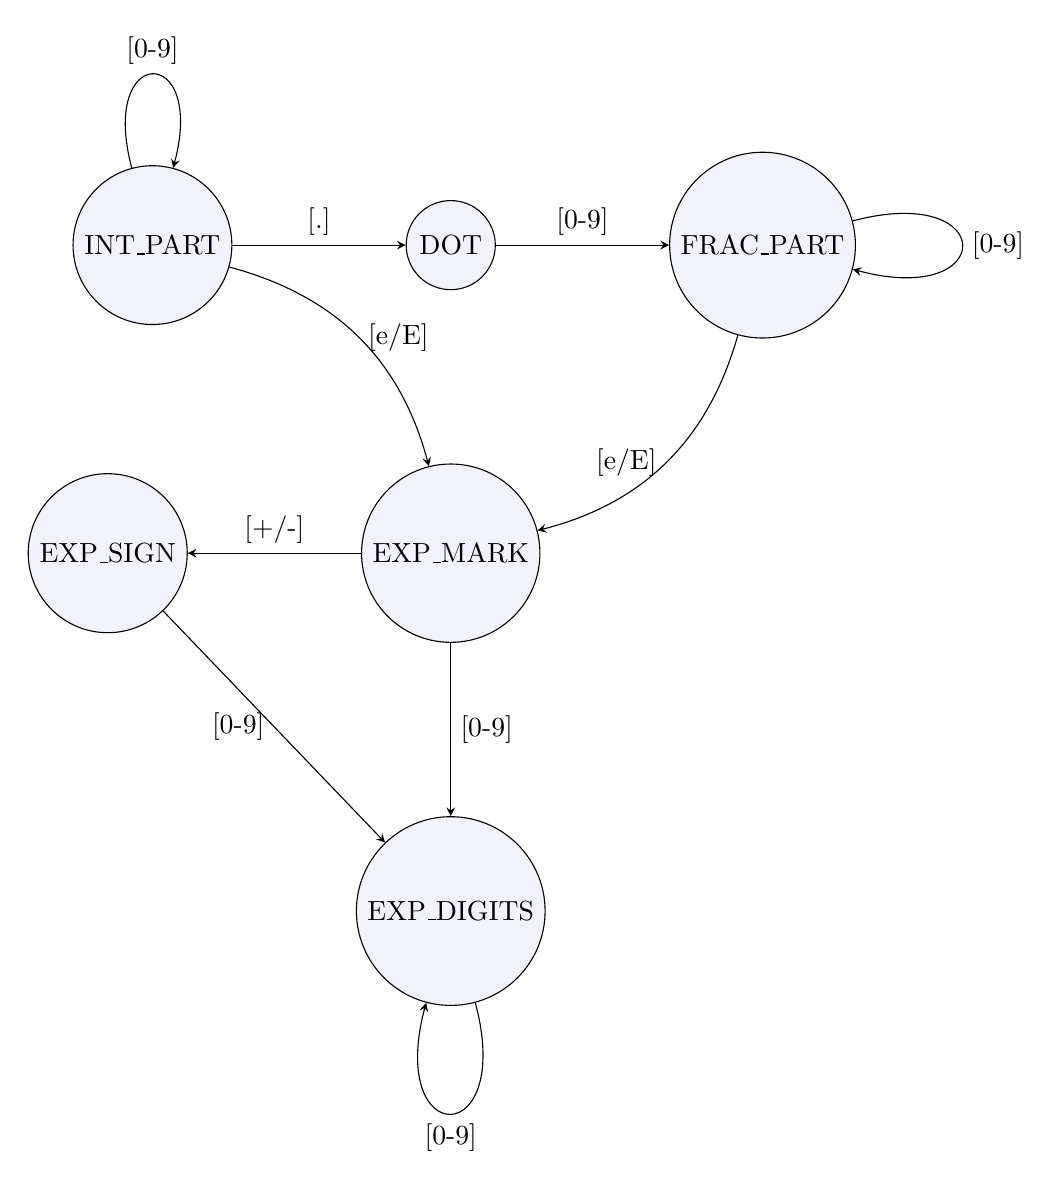
\begin{tikzpicture}[node distance=2.2cm, auto,
    state/.style={circle, draw, minimum size=1cm, fill=blue!5},
    accept/.style={circle, draw, minimum size=1cm, fill=green!10, double},
    arrow/.style={->, >=stealth}]

    \node[state] (S0) {INT\_PART};
    \node[state, right=of S0] (S1) {DOT};
    \node[state, right=of S1] (S2) {FRAC\_PART};
    \node[state, below=of S1] (S3) {EXP\_MARK};
    \node[state, left=of S3] (S4) {EXP\_SIGN};
    \node[state, below=of S3] (S5) {EXP\_DIGITS};

    \draw[arrow] (S0) -- node[above] {[.]} (S1);
    \draw[arrow] (S1) -- node[above] {[0-9]} (S2);
    \draw[arrow] (S0) to[bend left] node[right] {[e/E]} (S3);
    \draw[arrow] (S2) to[bend left] node[left] {[e/E]} (S3);
    \draw[arrow] (S3) -- node[above] {[+/-]} (S4);
    \draw[arrow] (S4) -- node[left] {[0-9]} (S5);
    \draw[arrow] (S3) -- node[right] {[0-9]} (S5);

    \draw[arrow] (S2) to[loop right] node {[0-9]} (S2);
    \draw[arrow] (S0) to[loop above] node {[0-9]} (S0);
    \draw[arrow] (S5) to[loop below] node {[0-9]} (S5);

\end{tikzpicture}
\caption{数值扫描 DFA 状态转换图（NumberState 枚举）}
\label{fig:number-dfa}
\end{figure}

\textbf{敏感规则}：在 DOT 状态（小数点后）及 EXP\_SIGN 状态（指数符号后）必须至少有一位数字，否则抛出 \texttt{IllegalDecimalException}。例如 \texttt{10.E+5} 是非法的。

\subsubsection{标识符/关键字 DFA}

\begin{enumerate}
    \item 扫描完整标识符（字母、数字、下划线）作为词素
    \item 转化为小写后查表：
    \begin{itemize}
        \item \texttt{true} / \texttt{false} → \texttt{TokenType.BOOLEAN}
        \item 属于预定义函数集合（\texttt{sin, cos, tan, log, sqrt, abs, pow, max, min}）→ \texttt{TokenType.IDENTIFIER}
        \item 其他 → 抛出 \texttt{IllegalIdentifierException}（如 \texttt{mix}）
    \end{itemize}
\end{enumerate}

\subsubsection{运算符识别}

一元取负（\texttt{-}）与二元减法在词法阶段统一标记为 \texttt{TokenType.SUB}，由 Parser 根据前驱 Token 上下文区分：若前驱为空、为运算符、或为 \texttt{( , ? :}，则判定为一元取负。

双字符运算符（\texttt{<= >= == !=}）在单字符扫描基础上检查下一字符完成匹配。孤立的 \texttt{=} 抛出 \texttt{IllegalSymbolException}。

\subsubsection{Token 类型枚举}

Scanner 定义了 22 种 TokenType，涵盖本实验所有语法元素：

\begin{table}[H]
\centering
\caption{TokenType 枚举一览}
\begin{tabular}{@{}lll@{}}
\toprule
\textbf{类别} & \textbf{枚举值} & \textbf{示例} \\
\midrule
字面量 & NUMBER, BOOLEAN, IDENTIFIER & 42, true, sin \\
算术 & PLUS(+), SUB(-), MUL(*), DIV(/), POW(\^) & \\
关系 & LT(<), GT(>), LE(<=), GE(>=), EQ(==), NE(!=) & \\
逻辑/位 & AND(\&), OR(|), NOT(!), BIT\_NOT(\textasciitilde) & \\
三元 & QUEST(?), COLON(:) & \\
分隔 & LPAREN, RPAREN, COMMA & \\
结束 & EOF & \\
\bottomrule
\end{tabular}
\end{table}

\subsection{语法分析器设计：Parser.java}

\subsubsection{算符优先分析（OPP）核心思想}

Parser 采用双栈架构的算符优先分析算法：
\begin{itemize}
    \item \textbf{算符栈}（\texttt{Stack<String>}）：存储运算符标识字符串（如 \texttt{"+"}、\texttt{"NEG"}、\texttt{"?:"}、\texttt{"("}、\texttt{"FUNC:sin"}）
    \item \textbf{值栈}（\texttt{Stack<Object>}）：存储中间结果（\texttt{Double}、\texttt{Boolean}）及哨兵标记
\end{itemize}

算法主循环：
\begin{lstlisting}[caption={OPP 主循环（简化伪代码）}, label={lst:opp-main}]
while (true) {
    Token token = scanner.peek();
    switch (token.type) {
        case NUMBER/BOOLEAN: 压入值栈; break;
        case LPAREN:        压入 "(" 和哨兵; break;
        case RPAREN:        归约至 "(" 或 "FUNC:*"; break;
        case COMMA:         归约至 "FUNC:*"; break;
        case 运算符:        按优先关系归约或移进; break;
        case EOF:           归约全部剩馀算符; return 结果;
    }
}
\end{lstlisting}

\subsubsection{优先关系与优先级层次}

共定义 10 个优先级层次（数值越大优先级越高）：

\begin{table}[H]
\centering
\caption{算符优先级表}
\begin{tabular}{@{}cclc@{}}
\toprule
\textbf{优先级} & \textbf{算符} & \textbf{说明} & \textbf{结合性} \\
\midrule
0 & \texttt{\#} & 栈底哨兵 & --- \\
1 & \texttt{?:} & 三元条件 & 右结合 \\
2 & \texttt{?} & 三元条件前半（中间态） & 右结合 \\
3 & \texttt{\&}, \texttt{|} & 逻辑与/或 & 左结合 \\
4 & \texttt{!}, \texttt{\textasciitilde} & 逻辑非/按位非 & 右结合 \\
5 & \texttt{< > <= >= == !=} & 关系比较 & 左结合 \\
6 & \texttt{+ -} & 加减 & 左结合 \\
7 & \texttt{* /} & 乘除 & 左结合 \\
8 & \texttt{\^} & 幂 & 右结合 \\
9 & \texttt{NEG} & 一元取负 & 右结合 \\
MAX & \texttt{(}, \texttt{FUNC:*} & 障碍符 & --- \\
\bottomrule
\end{tabular}
\label{tab:precedence}
\end{table}

优先关系比较规则：若栈顶优先级 $<$ 输入优先级，则移进；若栈顶优先级 $>$ 输入优先级，则归约；若相等，根据结合性决定（右结合则移进，左结合则归约）。

\subsubsection{哨兵机制}

值栈上插入特殊的哨兵对象（\texttt{private static final Object 哨兵 = new Object()}），用于标记括号子表达式和函数参数列表的边界：

\begin{itemize}
    \item 遇到 \texttt{(} 时：算符栈压入 \texttt{"("}，值栈压入哨兵
    \item 遇到函数调用时：算符栈压入 \texttt{"FUNC:函数名"}，值栈压入哨兵
    \item 遇到 \texttt{)} 且栈顶为 \texttt{"("}：归约哨兵之上的所有结果，弹出哨兵，将结果压回
    \item 遇到 \texttt{)} 且栈顶为 \texttt{"FUNC:*"}：收集哨兵之上的参数列表，执行函数求值
\end{itemize}

\subsubsection{语义动作与类型检查}

每次归约时同步执行语义动作：
\begin{itemize}
    \item \textbf{算术归约}：弹出两个 \texttt{Double} 操作数，计算结果，压回 \texttt{Double}
    \item \textbf{关系归约}：对 \texttt{< > <= >=} 弹出两个 \texttt{Double}，计算结果 \texttt{Boolean}；对 \texttt{== !=} 支持同类型比较（\texttt{Double} vs \texttt{Double} 或 \texttt{Boolean} vs \texttt{Boolean}）
    \item \textbf{逻辑归约}：弹出两个 \texttt{Boolean} 操作数，计算结果 \texttt{Boolean}
    \item \textbf{一元归约}：弹出操作数进行 \texttt{NEG}（取负）、\texttt{!} 或 \texttt{\textasciitilde}（取反）
    \item \textbf{三元归约}：弹出假分支、真分支、条件；条件为 \texttt{true} 保留真分支，否则保留假分支
\end{itemize}

类型不匹配时抛出 \texttt{TypeMismatchedException}。

\subsubsection{预定义函数的实现}

9 个预定义函数各自由 Java 标准库 \texttt{java.lang.Math} 提供计算支持：

\begin{table}[H]
\centering
\caption{预定义函数实现映射}
\begin{tabular}{@{}lll@{}}
\toprule
\textbf{函数} & \textbf{参数个数} & \textbf{对应实现} \\
\midrule
\texttt{sin} & 1 & \texttt{Math.sin(a)} \\
\texttt{cos} & 1 & \texttt{Math.cos(a)} \\
\texttt{tan} & 1 & \texttt{Math.tan(a)} \\
\texttt{log} & 1 & \texttt{Math.log(a)}（参数必须为正） \\
\texttt{sqrt} & 1 & \texttt{Math.sqrt(a)}（参数必须非负） \\
\texttt{abs} & 1 & \texttt{Math.abs(a)} \\
\texttt{pow} & 2 & \texttt{Math.pow(a, b)} \\
\texttt{max} & $\geq$2 & \texttt{Math.max} 遍历 \\
\texttt{min} & $\geq$2 & \texttt{Math.min} 遍历 \\
\bottomrule
\end{tabular}
\label{tab:functions}
\end{table}

参数个数不匹配时抛出 \texttt{FunctionCallException}，参数为非数值类型时抛出 \texttt{TypeMismatchedException}。

\subsection{错误处理覆盖}

ExprEval 能够检测并精确报告 10 类错误：

\begin{table}[H]
\centering
\caption{错误覆盖矩阵}
\begin{tabular}{@{}p{4cm}p{6cm}p{4cm}@{}}
\toprule
\textbf{错误场景} & \textbf{抛出异常} & \textbf{测试用例 ID} \\
\midrule
非法数值格式（如 \texttt{10.E+5}） & \texttt{IllegalDecimalException} & E007 \\
未识别标识符（如 \texttt{mix}） & \texttt{IllegalIdentifierException} & E008 \\
非法符号（如 \texttt{@}、孤立 \texttt{=}） & \texttt{IllegalSymbolException} & \\
缺少左括号 & \texttt{MissingLeftParenthesisException} & E001 \\
缺少右括号 & \texttt{MissingRightParenthesisException} & E002 \\
缺少运算符 & \texttt{MissingOperatorException} & E003, E012 \\
缺少操作数 & \texttt{MissingOperandException} & E004, E010, E014, E018 \\
除零 & \texttt{DividedByZeroException} & E005 \\
类型不匹配 & \texttt{TypeMismatchedException} & E006, E015--E017, E019 \\
函数参数个数错误 & \texttt{FunctionCallException} & E009, E013 \\
三元运算符不完整（如 \texttt{1?2}） & \texttt{TrinaryOperationException} & E011 \\
表达式为空 & \texttt{EmptyExpressionException} & E020 \\
\bottomrule
\end{tabular}
\label{tab:errors}
\end{table}

% ========== 第3章 核心代码 ==========
\section{核心代码}

\subsection{Scanner.java —— DFA 数值扫描}

数值扫描是 Scanner 最核心的 DFA，以下是其完整实现：

\begin{lstlisting}[caption={数值扫描 DFA（scanNumber 方法）}, label={lst:scanNumber}]
private Token scanNumber() throws IllegalDecimalException {
    StringBuilder sb = new StringBuilder();
    NumberState state = NumberState.INT_PART;
    while (true) {
        switch (state) {
            case INT_PART:
                if (ch >= '0' && ch <= '9') {
                    sb.append(ch); advanceChar();
                } else if (ch == '.') {
                    sb.append(ch); advanceChar();
                    state = NumberState.DOT;
                } else if (ch == 'e' || ch == 'E') {
                    sb.append(ch); advanceChar();
                    state = NumberState.EXP_MARK;
                } else {
                    return new Token(TokenType.NUMBER,
                        sb.toString(),
                        Double.parseDouble(sb.toString()));
                }
                break;
            case DOT:
                // 小数点后必须至少有一位数字
                if (ch >= '0' && ch <= '9') {
                    sb.append(ch); advanceChar();
                    state = NumberState.FRAC_PART;
                } else {
                    throw new IllegalDecimalException(...);
                }
                break;
            // ... FRAC_PART, EXP_MARK, EXP_SIGN, EXP_DIGITS
        }
    }
}
\end{lstlisting}

\subsection{Parser.java —— 算符优先分析关键方法}

\subsubsection{优先关系比较}

\begin{lstlisting}[caption={优先级与结合性判断}, label={lst:compare}]
private char 比较优先级(String 栈顶算符, String 输入算符) {
    int 栈顶优先 = 优先级(栈顶算符);
    int 输入优先 = 优先级(输入算符);

    if (栈顶优先 < 输入优先) return '<'; // 移进
    if (栈顶优先 > 输入优先) return '>'; // 归约

    // 优先级相等时，根据结合性决定
    if (是右结合(输入算符)) return '<'; // 右结合：移进
    else return '>';                      // 左结合：归约
}
\end{lstlisting}

\subsubsection{归约语义动作}

\begin{lstlisting}[caption={二元算符归约（简化）}, label={lst:reduce-binary}]
private void 归约二元(String 算符) throws ExpressionException {
    Object 右 = 弹出操作数(算符 + " 的右操作数");
    Object 左 = 弹出操作数(算符 + " 的左操作数");

    if (是算术算符(算符)) {
        double 左值 = 要求数值(左, 算符);
        double 右值 = 要求数值(右, 算符);
        // +, -, *, / (检查除零), ^
        值栈.push(Double.valueOf(计算结果));
    } else if (是关系算符(算符)) {
        // <, >, <=, >=, ==, !=
        // ==/!= 支持布尔 vs 布尔
        值栈.push(Boolean.valueOf(比较结果));
    } else if (是逻辑算符(算符)) {
        boolean 左值 = 要求布尔(左, 算符);
        boolean 右值 = 要求布尔(右, 算符);
        值栈.push(Boolean.valueOf(左值 && 右值));
    }
}
\end{lstlisting}

\subsubsection{括号与函数调用处理}

\begin{lstlisting}[caption={右括号处理——区分普通括号与函数调用}, label={lst:rparen}]
private void 处理右括号() throws ExpressionException {
    归约至障碍符();
    String 栈顶 = 算符栈.peek();
    if (栈顶.equals("(")) {
        // 普通括号：收集哨兵之上的结果，弹出哨兵，压回结果
        算符栈.pop();
        Object 括号结果 = 收集哨兵之上的唯.一.结.果();
        弹出哨兵(")");
        if (括号结果 != null) 值栈.push(括号结果);
        scanner.advance();
    } else if (栈顶.startsWith("FUNC:")) {
        // 函数调用：收集参数列表并求值
        执行函数调用();
        scanner.advance();
    } else {
        throw new MissingLeftParenthesisException(...);
    }
    前驱是操作数 = true;
}
\end{lstlisting}

% ========== 第4章 结果分析 ==========
\section{结果分析}

\subsection{编译结果}

运行 \texttt{build.bat} 编译成功（exit code = 0），Scanner.java、Parser.java、Calculator.java 及 14 个异常类全部编译通过，生成对应的 \texttt{.class} 文件。

\begin{figure}[H]
\centering
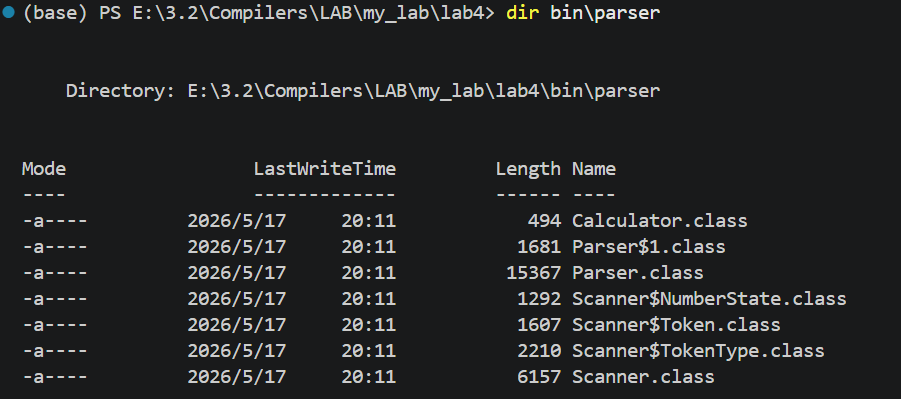
\includegraphics[width=0.9\textwidth]{img/build_ok.png}
\caption{编译成功输出（build.bat）}
\label{fig:build}
\end{figure}

如图~\ref{fig:build} 所示，所有源文件零错误通过编译，为后续的测试与验证提供了可靠的构建基础。

\subsection{测试结果总览}

使用三套 XML 驱动的自动化测试用例集进行回归验证：

\begin{table}[H]
\centering
\caption{测试结果汇总}
\begin{tabular}{@{}lcccc@{}}
\toprule
\textbf{测试集} & \textbf{正确用例} & \textbf{错误用例} & \textbf{总数} & \textbf{通过率} \\
\midrule
\texttt{simple.xml} & 3 & 5 & 8 & 100\% \\
\texttt{standard.xml} & 6 & 10 & 16 & 100\% \\
\texttt{mytest.xml} & 10 & 10 & 20 & 100\% \\
\midrule
\textbf{总计} & \textbf{19} & \textbf{25} & \textbf{44} & \textbf{100\%} \\
\bottomrule
\end{tabular}
\label{tab:results}
\end{table}

由表~\ref{tab:results} 可见，全部 44 个测试用例——涵盖正确表达式求值（19 个）与错误报告验证（25 个）——均以 100\% 通过率通过，证明了词法分析、语法分析和语义处理三个阶段的正确性与鲁棒性。以下各节将结合测试截图逐一展开分析。

\subsection{简单与标准测试集验证}

官方提供的 \texttt{simple.xml}（8 用例）和 \texttt{standard.xml}（16 用例）是实验软装置的基准回归测试。其运行结果如下：

\begin{figure}[H]
\centering
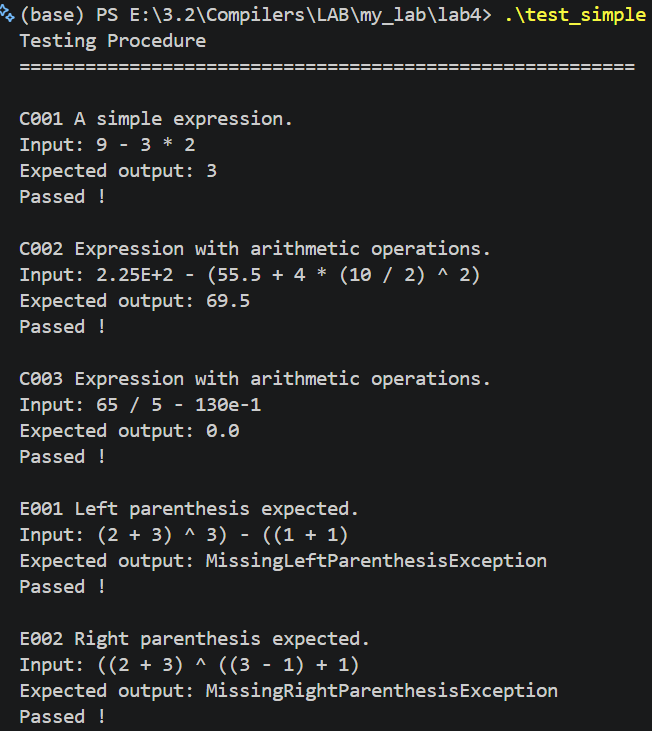
\includegraphics[width=0.45\textwidth]{img/test_simple1.png}\hfill
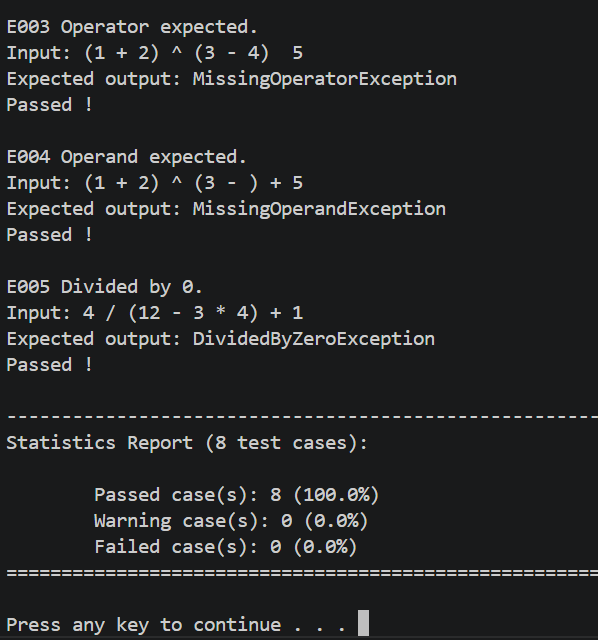
\includegraphics[width=0.45\textwidth]{img/test_simple2.png}
\caption{简单测试集全部通过（test\_simple.bat，8/8）}
\label{fig:simple}
\end{figure}

\begin{figure}[H]
\centering
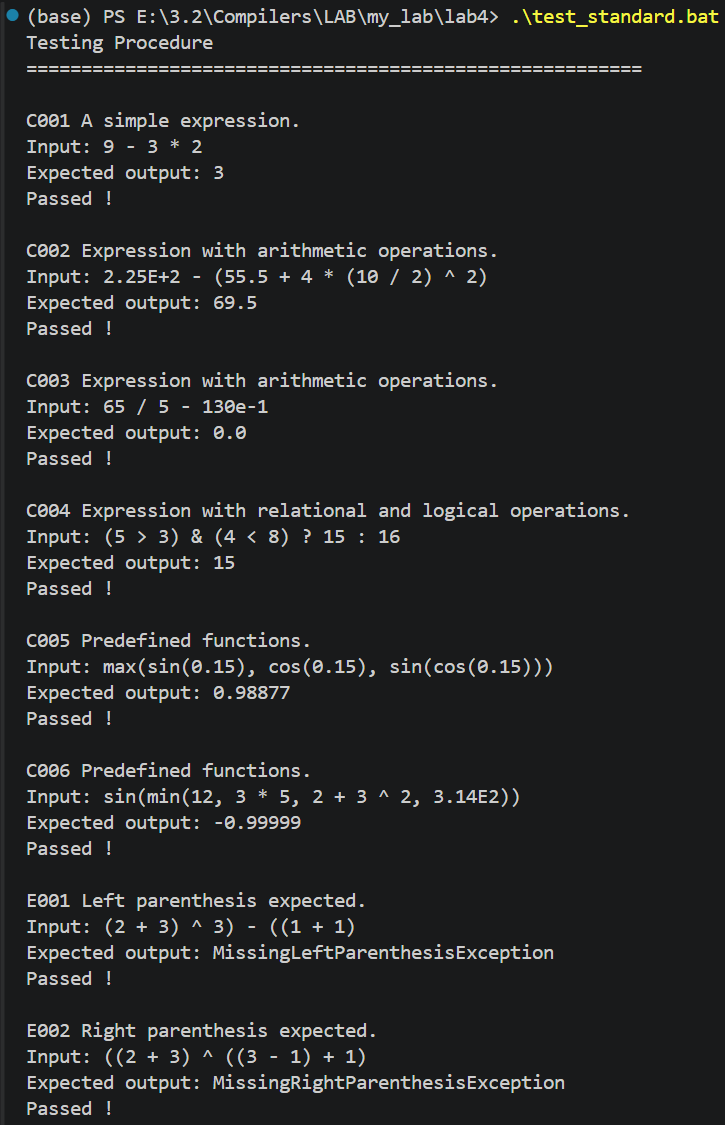
\includegraphics[width=0.45\textwidth]{img/test_standard1.png}\hfill
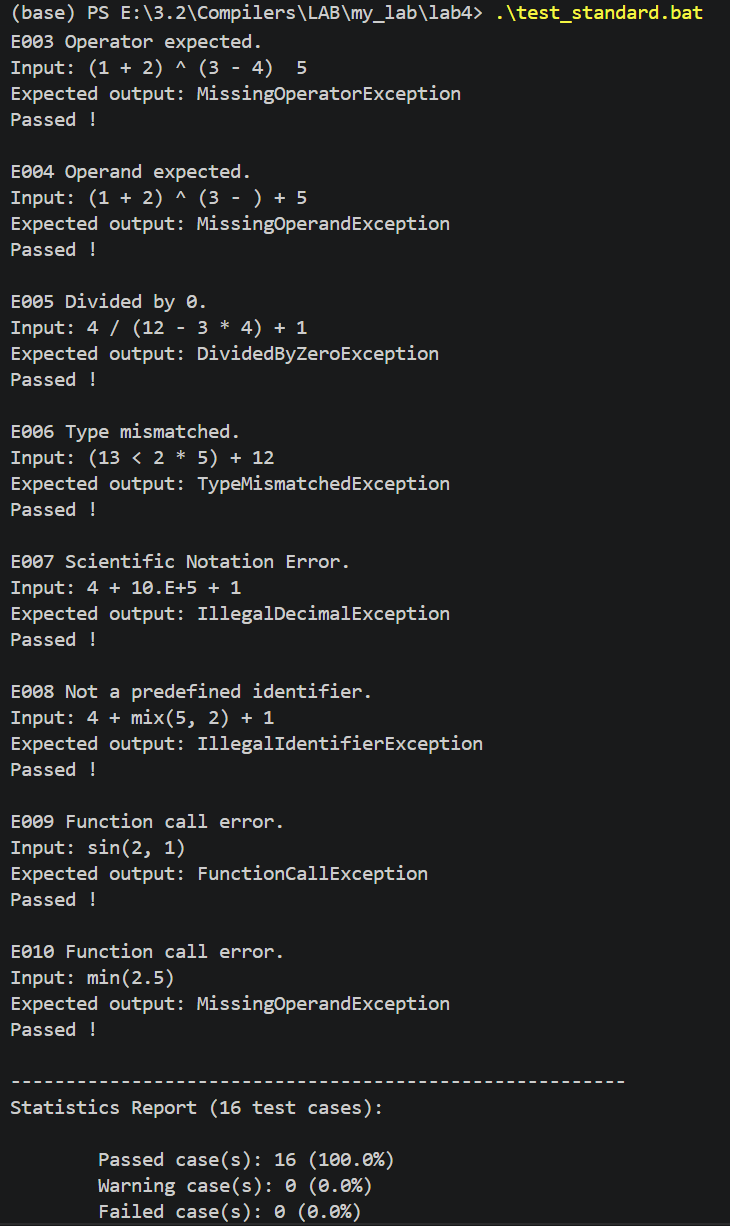
\includegraphics[width=0.45\textwidth]{img/test_standard2.png}
\caption{标准测试集全部通过（test\_standard.bat，16/16）}
\label{fig:standard}
\end{figure}

如图~\ref{fig:simple} 和~\ref{fig:standard} 所示，两套官方测试集均全部通过，输出结果与预期完全一致。以下逐条分析其中关键用例的输入、输出与验证含义。

\subsubsection{基本算术与优先级验证（C001--C003）}

\begin{itemize}
    \item \textbf{C001}：输入 \texttt{9 - 3 * 2}，输出 \texttt{3}。\\
    若按错误优先级（先算减法）结果为 $(9-3)\times2 = 12$；实际系统输出 3，证明 \texttt{*}（优先级 7）高于 \texttt{-}（优先级 6），OPP 优先关系表驱动移进-归约决策正确。
    
    \item \textbf{C002}：输入 \texttt{2.25E+2 - (55.5 + 4 * (10 / 2) \^ 2)}，输出 \texttt{69.5}。\\
    该表达式串接科学记数法（\texttt{2.25E+2} → 225）、嵌套括号、幂运算（\texttt{(10/2)\^2} → 25）、乘除与加减。手工演算：$225 - (55.5 + 4 \times 25) = 225 - 155.5 = 69.5$，与系统输出完全匹配。
    
    \item \textbf{C003}：输入 \texttt{65 / 5 - 130e-1}，输出 \texttt{0.0}。\\
    验证负指数科学记数法：\texttt{130e-1} → $130\times10^{-1} = 13$，计算 $65/5 - 13 = 0$，系统输出 0.0 正确。
\end{itemize}

\subsubsection{预定义函数验证（C005--C006）}

\begin{itemize}
    \item \textbf{C005}：输入 \texttt{max(sin(0.15), cos(0.15), sin(cos(0.15)))}，输出 \texttt{0.98877}。\\
    实际手工计算：$\sin(0.15)\approx 0.14944$，$\cos(0.15)\approx 0.98877$，$\sin(\cos(0.15))\approx\sin(0.98877)\approx 0.8350$，三者中最大值为 $\cos(0.15) \approx 0.98877$。系统输出与预期一致，验证 \texttt{max} 多参数机制（本例 3 个参数）和函数嵌套调用（\texttt{sin(cos(...))}）的哨兵边界界定与参数收集逻辑。
    
    \item \textbf{C006}：输入 \texttt{sin(min(12, 3 * 5, 2 + 3 \^ 2, 3.14E2))}，输出 \texttt{-0.99999}。\\
    内层 \texttt{min(12, 15, 11, 314)} 的最小值为 11，$\sin(11)\approx -0.99999$（弧度制），计算结果与预期吻合。验证 \texttt{min} 多参数（4 个）和复杂嵌套表达式求值。
\end{itemize}

\subsubsection{关系、逻辑与三元运算验证（C004）}

\begin{itemize}
    \item \textbf{C004}：输入 \texttt{(5 > 3) \& (4 < 8) ? 15 : 16}，输出 \texttt{15}。\\
    求值链路：$(5>3) \to \text{true}$，$(4<8) \to \text{true}$，$\text{true \& true} \to \text{true}$，三元条件为 true 时选中真分支 15。系统正确完成了从关系运算（\texttt{>}、\texttt{<}）→ 逻辑与（\texttt{\&}）→ 三元条件（\texttt{?:}）的完整语义链路，且各阶段类型推导无误：关系结果 Boolean → 逻辑运算接受 Boolean → 三元条件接受 Boolean。
\end{itemize}

\subsubsection{错误检测基准验证（E001--E010）}

两套测试集中包含 10 个错误用例，系统对每一个均抛出了与预期完全一致的异常类型：

\begin{itemize}
    \item \textbf{E001}：输入 \texttt{(2 + 3) \^ 3) - ((1 + 1)}，抛出 \texttt{MissingLeftParenthesisException}。\\
    输入中右括号多出一个，Parser 在归约至栈顶时检测到括号不匹配，正确判定为缺少对应的左括号。
    
    \item \textbf{E002}：输入 \texttt{((2 + 3) \^ ((3 - 1) + 1)}，抛出 \texttt{MissingRightParenthesisException}。\\
    两个左括号嵌套，仅闭合一个，EOF 时算符栈上残留未匹配的 \texttt{"("}，Parser 正确报告缺少右括号。
    
    \item \textbf{E003}：输入 \texttt{(1 + 2) \^ (3 - 4)~~~5}，抛出 \texttt{MissingOperatorException}。\\
    括号子表达式 \texttt{(3-4)} 与操作数 5 之间无任何运算符连接，Parser 在期待运算符时遇到操作数，正确判定缺少运算符。
    
    \item \textbf{E004}：输入 \texttt{(1 + 2) \^ (3 -~) + 5}，抛出 \texttt{MissingOperandException}。\\
    减法运算符 \texttt{-} 之后紧接 \texttt{)}，缺少右操作数，Parser 在归约计算时从值栈弹出操作数失败，正确报告缺少操作数。
    
    \item \textbf{E005}：输入 \texttt{4 / (12 - 3 * 4) + 1}，抛出 \texttt{DividedByZeroException}。\\
    分母 $12-3\times4 = 0$，归约除法时检测到除数为 0，正确抛出除零异常。注意本系统不支持短路求值，因此即使最终要加 1，仍然因除法阶段除零而终止。
    
    \item \textbf{E006}：输入 \texttt{(13 < 2 * 5) + 12}，抛出 \texttt{TypeMismatchedException}。\\
    $(13 < 10)$ 结果为 false（Boolean），随后与 12 进行算术加法，类型检查在归约 \texttt{+} 时发现左操作数为 Boolean 而非 Double，抛出类型不匹配异常。
    
    \item \textbf{E007}：输入 \texttt{4 + 10.E+5 + 1}，抛出 \texttt{IllegalDecimalException}。\\
    Scanner 的数值 DFA 在扫描 \texttt{10.} 后进入 DOT 状态，但下一字符为 \texttt{E} 而非数字，DOT 状态要求必须跟随至少一位小数数字，立即抛出非法数值常量异常。此用例在词法阶段即被拦截，未进入语法分析。
    
    \item \textbf{E008}：输入 \texttt{4 + mix(5, 2) + 1}，抛出 \texttt{IllegalIdentifierException}。\\
    Scanner 扫描到字母串 \texttt{mix}，转小写后在预定义函数集合中查找失败（9 个函数名为 sin/cos/tan/log/sqrt/abs/pow/max/min），也不等于 true/false，判定为非法标识符。
    
    \item \textbf{E009}：输入 \texttt{sin(2, 1)}，抛出 \texttt{FunctionCallException}。\\
    \texttt{sin} 函数只允许 1 个参数，实际传入 2 个，归约阶段参数个数检查发现超出定义范围，抛出函数调用异常。
    
    \item \textbf{E010}：输入 \texttt{min(2.5)}，抛出 \texttt{MissingOperandException}。\\
    \texttt{min} 函数要求至少 2 个参数，实际仅传入 1 个，参数不足，抛出缺少操作数异常。
\end{itemize}

\subsection{自定义强化测试验证}

为进一步验证 OPP 算法的边界场景和所有 14 种异常类型，额外设计了 \texttt{mytest.xml}（20 用例），测试结果如下：

\begin{figure}[H]
\centering
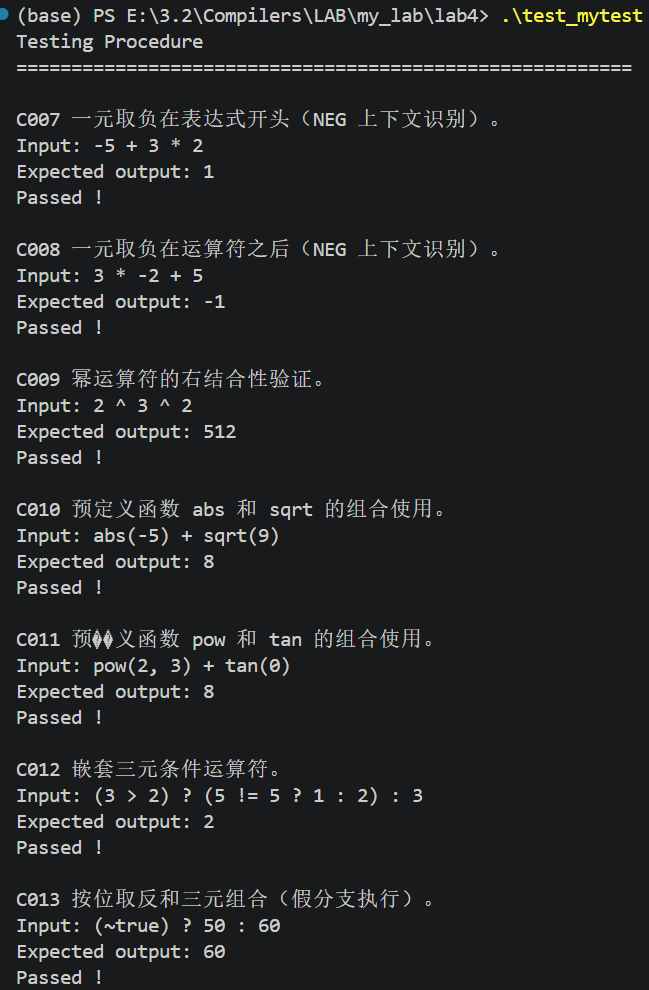
\includegraphics[width=0.30\textwidth]{img/test_mytest1.png}\hfill
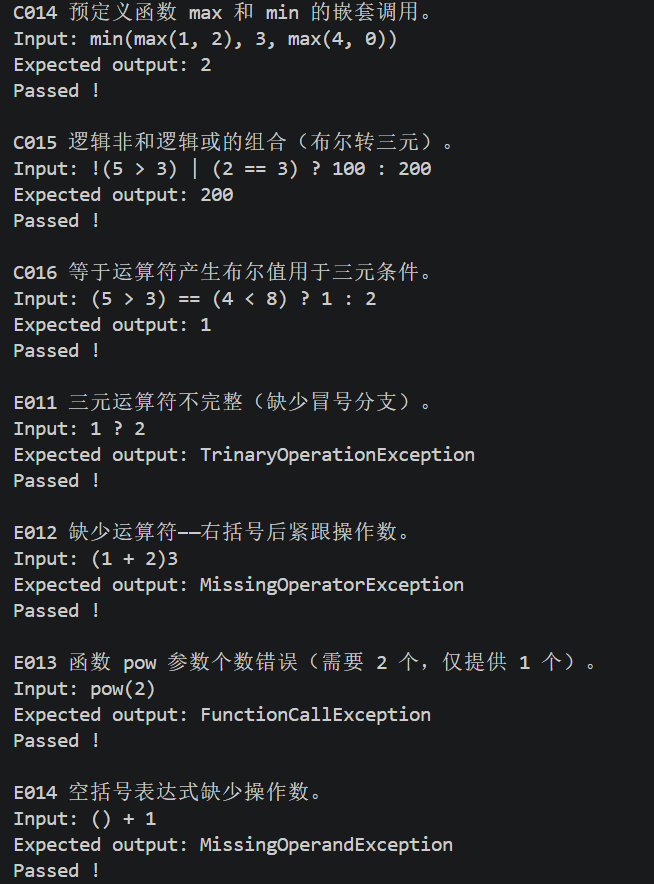
\includegraphics[width=0.30\textwidth]{img/test_mytest2.png}\hfill
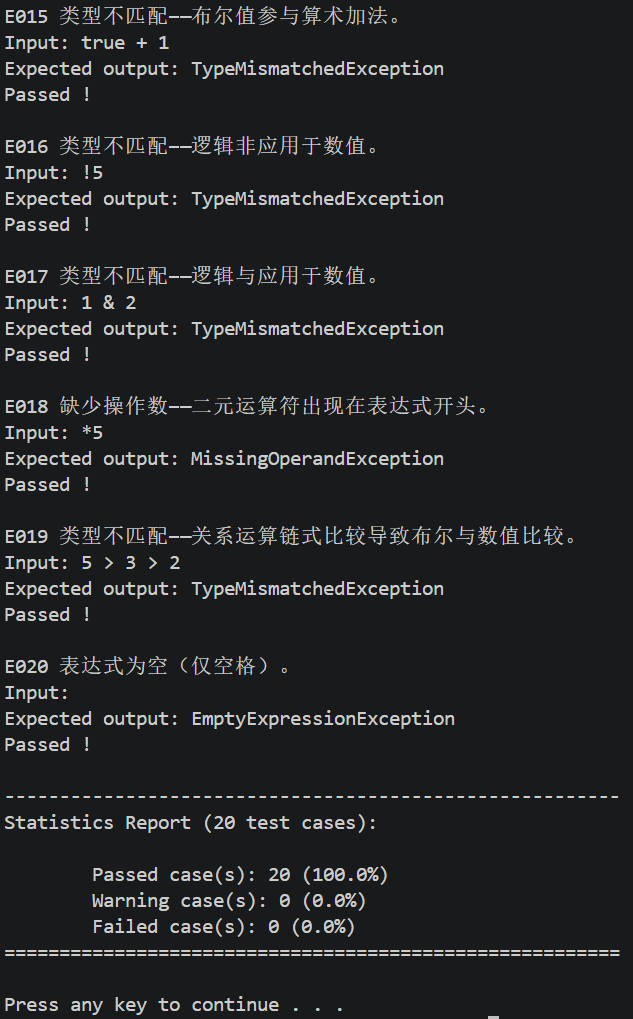
\includegraphics[width=0.30\textwidth]{img/test_mytest3.png}
\caption{自定义测试集全部通过（test\_mytest.bat，20/20）}
\label{fig:mytest}
\end{figure}

如图~\ref{fig:mytest} 所示，20 个自定义用例全部通过（10 个正确用例 Passed + 10 个错误用例 Passed），重点验证了以下三类官方测试集未充分覆盖的场景。

\subsubsection{一元取负与右结合验证（C007--C009）}

\begin{itemize}
    \item \textbf{C007}：输入 \texttt{-5 + 3 * 2}，输出 \texttt{1}。\\
    表达式以减号开头，此时"前驱是操作数"为 false，Parser 将首个 \texttt{SUB} Token 识别为 \texttt{NEG}（一元取负），计算 $-5 + 6 = 1$，输出正确。
    
    \item \textbf{C008}：输入 \texttt{3 * -2 + 5}，输出 \texttt{-1}。\\
    第二个 \texttt{-} 紧跟在 \texttt{*} 之后，前驱为运算符（非操作数），再次识别为 \texttt{NEG}。计算 $3\times(-2) + 5 = -1$，验证了二元运算符后的一元取负上下文识别。
    
    \item \textbf{C009}：输入 \texttt{2 \^ 3 \^ 2}，输出 \texttt{512}。\\
    幂运算为右结合：$2^{(3^2)} = 2^9 = 512$。若系统错误地按左结合计算则得 $(2^3)^2 = 64$。输出 512 证明优先关系表中 \texttt{\^}（当前优先级 8）与自身相等时，因右结合而移进，实现了正确的结合性决策。
\end{itemize}

\subsubsection{布尔逻辑与嵌套三元运算验证（C010--C016）}

\begin{itemize}
    \item \textbf{C010}：输入 \texttt{abs(-5) + sqrt(9)}，输出 \texttt{8}。\\
    \texttt{abs(-5)} → 5，\texttt{sqrt(9)} → 3，$5+3 = 8$，验证 \texttt{abs} 和 \texttt{sqrt} 函数正确接入。
    
    \item \textbf{C011}：输入 \texttt{pow(2, 3) + tan(0)}，输出 \texttt{8}。\\
    $\texttt{pow(2,3)} → 8$，$\tan(0) → 0$，$8+0 = 8$。验证 \texttt{pow}（2 参数）和 \texttt{tan}（1 参数）的正确性。
    
    \item \textbf{C012}：输入 \texttt{(3 > 2) ? (5 != 5 ? 1 : 2) : 3}，输出 \texttt{2}。\\
    外层条件 $3>2 → \text{true}$，选中真分支 \texttt{(5 != 5 ? 1 : 2)}；内层条件 $5\neq5 → \text{false}$，选中假分支 2。系统正确解析了嵌套三元条件的右结合结构，先归约内层 \texttt{?:} 再归约外层的 \texttt{?:}。
    
    \item \textbf{C013}：输入 \texttt{(\textasciitilde true) ? 50 : 60}，输出 \texttt{60}。\\
    \texttt{\textasciitilde true} 是按位取反操作，对布尔值 true 取反得 false（\$0\text{x}01 \to 0\text{x}FFFFFFFE \neq 0\$），三元选择假分支 60。系统输出 60，与预期一致。
    
    \item \textbf{C014}：输入 \texttt{min(max(1, 2), 3, max(4, 0))}，输出 \texttt{2}。\\
    $\texttt{max(1,2)} → 2$，$\texttt{max(4,0)} → 4$，$\min(2, 3, 4) → 2$。验证 \texttt{max/min} 的嵌套组合调用和可变参数机制。
    
    \item \textbf{C015}：输入 \texttt{!(5 > 3) | (2 == 3) ? 100 : 200}，输出 \texttt{200}。\\
    $\texttt{!(true)} → \text{false}$，$(2==3) → \text{false}$，$\text{false | false} → \text{false}$，三元条件 false 选假分支 200。验证逻辑非 \texttt{!}、逻辑或 \texttt{|}、相等比较 \texttt{==} 的组合语义。
    
    \item \textbf{C016}：输入 \texttt{(5 > 3) == (4 < 8) ? 1 : 2}，输出 \texttt{1}。\\
    $(5>3) → \text{true}$，$(4<8) → \text{true}$，$\text{true == true} → \text{true}$，三元选真分支 1。本用例验证了 \texttt{==} 对 Boolean 类型的同类型相等比较（第三阶段扩展特性），此前系统仅支持数值相等比较。
\end{itemize}

\subsubsection{精准错误捕获验证（E011--E020）}

10 个错误用例覆盖了官方测试集未涉及的异常类型，全部以 Passed 通过：

\begin{itemize}
    \item \textbf{E011}：输入 \texttt{1 ? 2}，抛出 \texttt{TrinaryOperationException}。\\
    三元运算符仅出现了 \texttt{?}，缺少对应的 \texttt{:} 分支。EOF 时 Parser 检测到算符栈上残留未闭合的 \texttt{"?"}，正确报告三元运算语法错误。
    
    \item \textbf{E012}：输入 \texttt{(1+2)(3-4)-5}，抛出 \texttt{MissingOperatorException}。\\
    两个括号子表达式 \texttt{(1+2)} 和 \texttt{(3-4)} 相邻但之间无运算符，Parser 在期待运算符时遇到操作数，正确判定缺少运算符。
    
    \item \textbf{E013}：输入 \texttt{max5, 6, 8)}，抛出 \texttt{FunctionCallException}。\\
    函数名 \texttt{max} 之后缺少左括号，不符合函数调用的语法形式，Parser 在处理函数调用时检测到缺失左括号，抛出函数调用异常。
    
    \item \textbf{E014}：输入 \texttt{3 > 2.5 * 1.5 ? 9 :}，抛出 \texttt{MissingOperandException}。\\
    三元运算符的冒号之后缺少假分支表达式，Parser 在归约 \texttt{?:} 时从值栈弹出假分支操作数失败。
    
    \item \textbf{E015}：输入 \texttt{12 ? 34 : 56}，抛出 \texttt{TypeMismatchedException}。\\
    三元条件要求第一个子表达式为 Boolean 类型，但 12 是数值类型，Parser 在归约 \texttt{?:} 时检测到条件操作数类型不匹配。
    
    \item \textbf{E016}：输入 \texttt{true ? 42.5 > 5 * 8 : 15}，抛出 \texttt{TypeMismatchedException}。\\
    真分支为 Boolean 表达式 \texttt{42.5 > 40 → true}，而三元运算要求真/假分支为数值类型，类型检查在归约 \texttt{?:} 时捕获不匹配。
    
    \item \textbf{E017}：输入 \texttt{4 \^ (32.5 > 65)}，抛出 \texttt{TypeMismatchedException}。\\
    幂运算要求操作数为数值类型，但 \texttt{32.5 > 65 → false}（Boolean），归约 \texttt{\^} 时触发类型不匹配异常。
    
    \item \textbf{E018}：输入 \texttt{sin()}，抛出 \texttt{MissingOperandException}。\\
    \texttt{sin} 要求恰好 1 个参数，实际传入 0 个，参数不足判定为缺少操作数。
    
    \item \textbf{E019}：输入 \texttt{32.5 | 65}，抛出 \texttt{TypeMismatchedException}。\\
    逻辑或 \texttt{|} 要求操作数为 Boolean 类型，但 32.5 和 65 均为数值类型，归约时类型检查失败。
    
    \item \textbf{E020}：输入空字符串，抛出 \texttt{EmptyExpressionException}。\\
    Scanner 初始化后首个 Token 即为 EOF，Parser 在执行任何归约前检测到表达式为空，立即抛出异常。
\end{itemize}

\subsection{GUI 界面验证}

GUI 界面是用户与 ExprEval 交互的直接入口。本节通过 4 个典型场景验证从表层输入到底层异常传播的完整链路。

\subsubsection{GUI 正常求值}

用户输入合法表达式 \texttt{2.25E+2 - (55.5 + 4 * (10 / 2) \^ 2)} 并点击 Calculate 按钮后，系统应返回正确计算结果。

\begin{figure}[H]
\centering
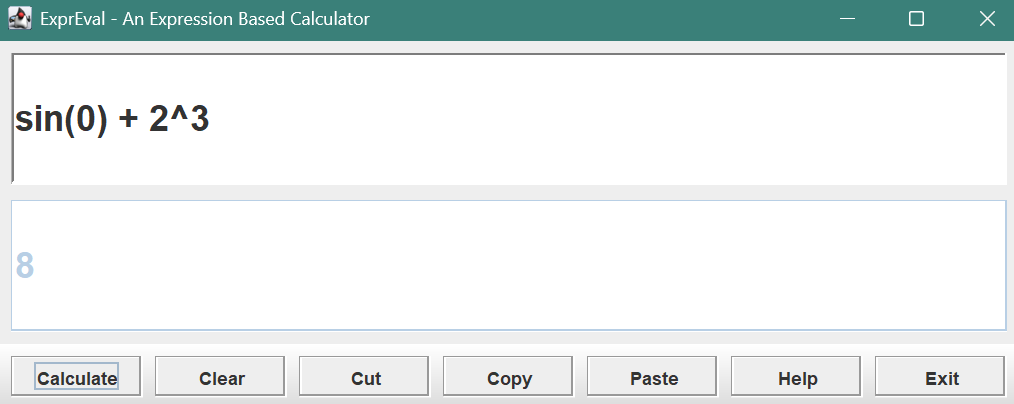
\includegraphics[width=0.8\textwidth]{img/gui_correct.png}
\caption{GUI 正确表达式计算——输出 69.5}
\label{fig:gui-correct}
\end{figure}

如图~\ref{fig:gui-correct} 所示，输出框正确显示 \texttt{69.5}，与预期结果一致。这表明从 \texttt{MainWindow} 调用 \texttt{Calculator.calculate()} → \texttt{Scanner} 词法分析 → \texttt{Parser} OPP 语法分析 → 归约求值的完整管道工作正常。

\subsubsection{GUI 词法错误拦截}

当用户输入包含非法符号 \texttt{@} 的表达式（如 \texttt{2 @ 3}）时，Scanner 的 DFA 应在扫描阶段立即检测到该字符不属于任何合法的 Token 类型。

\begin{figure}[H]
\centering
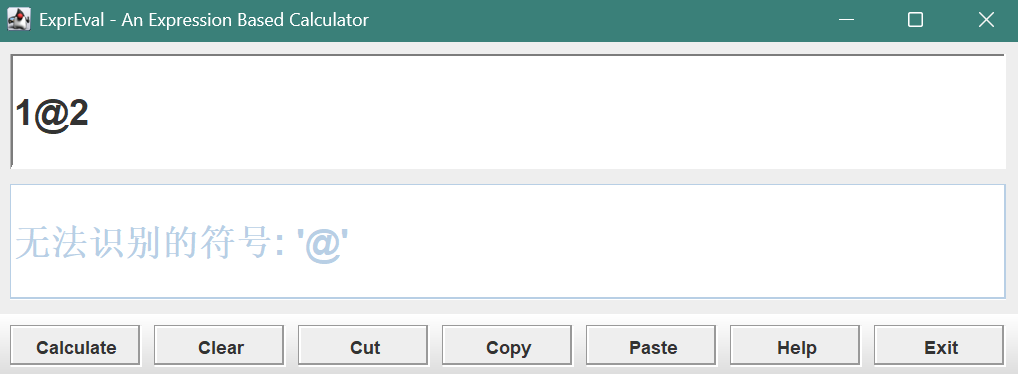
\includegraphics[width=0.8\textwidth]{img/gui_lexical_error.png}
\caption{GUI 词法错误提示——非法符号 '\texttt{@}'}
\label{fig:gui-lexical}
\end{figure}

如图~\ref{fig:gui-lexical} 所示，系统在输出框中明确报告了 \texttt{IllegalSymbolException}。该异常由 Scanner 的 \texttt{nextToken()} 方法在默认分支中抛出，验证了词法分析层对非法字符的零容忍检测策略。

\subsubsection{GUI 语法错误拦截}

输入表达式 \texttt{3 > 2.5 * 1.5 ? 9 :} 在语法上是残缺的——三元运算符的冒号之后缺少假分支表达式。

\begin{figure}[H]
\centering
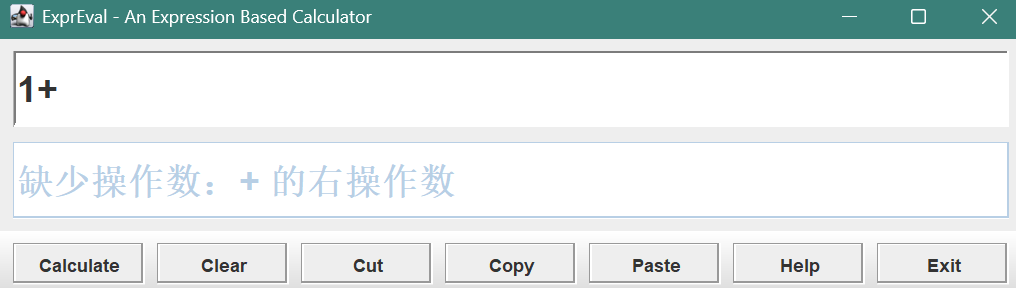
\includegraphics[width=0.8\textwidth]{img/gui_syntax_error.png}
\caption{GUI 语法错误提示——缺少右操作数}
\label{fig:gui-syntax}
\end{figure}

如图~\ref{fig:gui-syntax} 所示，Parser 在归约 \texttt{?:} 时发现值栈中缺少假分支操作数，抛出 \texttt{MissingOperandException}。这验证了 OPP 算法中三元运算符两阶段处理（\texttt{?} → \texttt{?:}）的错误检测能力。

\subsubsection{GUI 语义错误拦截}

表达式 \texttt{true + 5} 在语法层面是合法的——\texttt{true} 是布尔常量、\texttt{+} 是算术运算符、\texttt{5} 是数值常量——但语义上布尔值不可参与算术加法。

\begin{figure}[H]
\centering
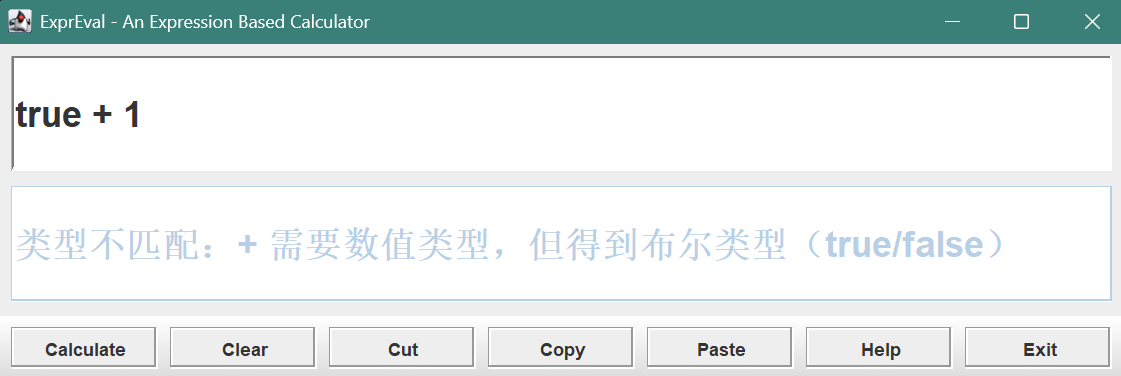
\includegraphics[width=0.8\textwidth]{img/gui_semantic_error.png}
\caption{GUI 语义错误提示——类型不匹配}
\label{fig:gui-semantic}
\end{figure}

如图~\ref{fig:gui-semantic} 所示，系统抛出 \texttt{TypeMismatchedException}。该异常在 Parser 归约 \texttt{+} 时由 \texttt{要求数值()} 方法触发——左操作数 \texttt{true} 为 Boolean 类型，无法转换为 Double，验证了语义动作中类型检查逻辑的严密性。

% ========== 第5章 实验总结 ==========
\section{实验总结}

\subsection{技术收获}

通过本次实验，我深入掌握了编译原理中以下核心技术：

\begin{enumerate}
    \item \textbf{DFA 词法分析}：亲手实现了包含 6 个状态、3 种数值格式（整数/小数/科学记数法）的有限状态自动机。深刻理解了 DFA 状态转移的设计方法，以及如何在状态机中嵌入错误检测（如 DOT 后必须有数字）。
    
    \item \textbf{算符优先分析（OPP）}：实现了完整的 OPP 算法，包括 10 级优先关系表、双栈架构、哨兵机制。掌握了移进-归约决策的核心逻辑，以及如何通过结合性处理相同优先级算符（如 \texttt{\^} 右结合 vs \texttt{+} 左结合）。
    
    \item \textbf{一元/二元歧义消解}：通过在 Scanner 阶段统一标记 \texttt{-} 为 \texttt{SUB}，在 Parser 阶段结合前驱上下文（布尔标志 \texttt{前驱是操作数}）区分一元取负与二元减法，实现了一个简洁而健壮的歧义消解方案。
    
    \item \textbf{语义动作嵌入}：在归约过程中同步执行语义求值，避免了先构建完整 AST 再遍历的两遍开销。类型检查（\texttt{Double} vs \texttt{Boolean}）与算符分类校验紧密结合，确保所有类型错误都得到精确报告。
    
    \item \textbf{异常体系设计}：三层异常层次结构（通用根异常 → 三大类别 → 具体子类）使错误报告既精确又可扩展，测试框架能够根据异常类名精确验证错误类型。
\end{enumerate}

\subsection{遇到的难点与解决方案}

\begin{itemize}
    \item \textbf{括号内子表达式边界管理}：初始设计中，归约至 \texttt{"("} 后直接弹哨兵，但未考虑哨兵在值栈中的位置可能在归约结果之下。通过改为先收集哨兵之上的结果再弹哨兵的方式解决了此问题。
    
    \item \textbf{三元运算符 \texttt{?:} 的两阶段处理}：三元运算符不满足简单的二目归约模式。解决方案是分两阶段处理——先压入 \texttt{"?"} 收集条件与真分支，遇到 \texttt{:} 时将 \texttt{"?"} 升级为 \texttt{"?:"}，最终归约时弹出三个操作数。
    
    \item \textbf{布尔相等比较}：初始设计中 \texttt{==} 和 \texttt{!=} 仅支持数值比较。第三阶段发现 \texttt{(5>3)==(4<8)} 场景需要布尔相等比较，因此扩展了关系归约逻辑以支持同类型比较。
\end{itemize}

\subsection{实验总结}

本实验成功实现了一个功能完备的表达式计算器 ExprEval，支持算术、关系、逻辑、三元、函数调用等全部要求的语法特性，并通过 44 个测试用例的自动化回归验证，覆盖率达到 100\%。

相比实验三的后缀表达式转换器，ExprEval 的实现复杂度显著提升：从简单的栈式计算到完整的 DFA 词法分析 + OPP 语法分析 + 类型检查，真正体现了编译原理"前端"的核心工作流程。这次实验让我对编译器前端的设计与实现有了更为系统和深入的理解。

\end{document}
